\documentclass{article}
\usepackage[a4paper, margin=2.5cm]{geometry}
\usepackage{amsmath, amssymb}
\usepackage[utf8]{inputenc}
\usepackage[dvipsnames]{xcolor}
\usepackage{tikz}

\title{Initial Progress Report}
\author{Haya Al-Kuwari, Akhyar Kamili, Abubaker Omer, Mohammed Nurul Hoque}
\date{\today}

\begin{document}
    \maketitle
    \hrule\relax
    \section{The Pipeline}
    \begin{center}
        
        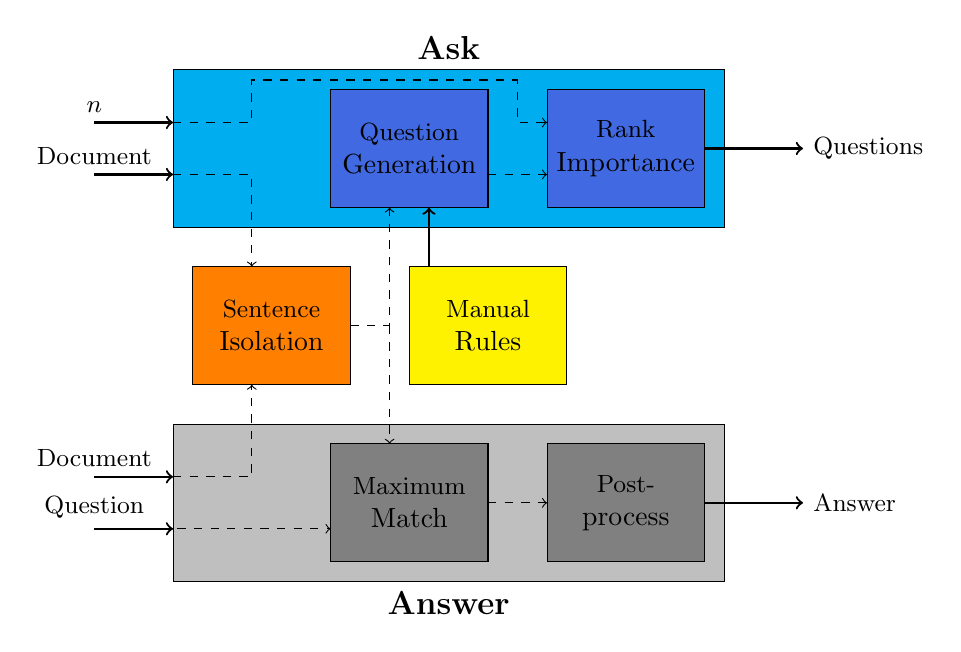
\begin{tikzpicture}
            \draw[fill=lightgray] (1,0) rectangle(8,2);
            \node[below] at (4.5,0) {\large\bfseries Answer};
            \draw[fill=orange] (1.25,2.5) rectangle (3.25,4);
            \node[align=center] at (2.25, 3.25) {\small Sentence\\Isolation};
            \draw[fill=cyan] (1, 4.5) rectangle (8,6.5);
            \node[above] at (4.5,6.5) {\large\bfseries Ask};
            % Input
            \draw[thick,->] (0, 0.67) node[above] {\small Question} -- (1, 0.67);
            \draw[thick,->] (0, 1.33) node[above] {\small Document} -- (1, 1.33);
            \draw[thick,->] (0, 5.17) node[above] {\small Document} -- (1, 5.17);
            \draw[thick,->] (0, 5.83) node[above] {\small $n$} -- (1, 5.83);
            % to sent. isolation
            \draw[dashed,->] (1,1.33) -- (2,1.33) -- (2,2.5);
            \draw[dashed,->] (1,5.17) -- (2,5.17) -- (2, 4);
            % out sent. isolation
            \draw[dashed,->] (3.25,3.25) -- (3.75,3.25) -- (3.75,4.75);
            \draw[dashed,->] (3.75,3.25) -- (3.75,1.75);
            % Maximum match
            \draw[fill=gray] (3,0.25) rectangle (5,1.75);
            \node[align=center] at (4,1) {\small Maximum\\Match};
            % Post process
            \draw[fill=gray] (5.75,0.25) rectangle (7.75,1.75);
            \draw[dashed,->] (0,0.67) -- (3,0.67);
            \node[align=center] at (6.75,1) {\small Post-\\process};
            \draw[dashed,->] (5,1) -- (5.75,1);
            \draw[thick,->] (7.75,1) -- (9,1) node[right] {\small Answer};
            % Manual rules
            \draw[fill=yellow] (4,2.5) rectangle (6, 4);
            \node[align=center] at (5, 3.25) {\small Manual\\Rules};
            \draw[thick,->] (4.25,4) -- (4.25,4.75);
            % Question generation
            \draw[fill=RoyalBlue] (3,4.75) rectangle (5,6.25);
            \node[align=center] at (4,5.5) {\small Question\\Generation};
            % Rank importance
            \draw[fill=RoyalBlue] (5.75,4.75) rectangle (7.75,6.25);
            \node[align=center] at (6.75,5.5) {\small Rank\\Importance};
            \draw[dashed,->] (5,5.17) -- (5.75,5.17);
            \draw[thick,->] (7.75,5.5) -- (9,5.5) node[right] {\small Questions};
            % n to ranking
            \draw[dashed,->] (1,5.83) -- (2,5.83) -- (2,6.37) -- (5.37,6.37) -- (5.37,5.83) --
            (5.75,5.83);
        \end{tikzpicture}
    \end{center}
    \subsection{Sentence Isolation}
    Reference resolution and sentence segmentation so that each sentence is $\sim$independent. This
    should also remove parenthetical expressions and put them as standalone sentences.
    \subsection{Manual Rules}
    A set of manual rules for generating a question from a sentence (using parse tree?).
    \subsection{Questions Generation}
    Apply the rules on sentences to generate the questions (also maybe add random variations of each
    generated sentence).
    \subsection{Rank Importance}
    Rank all questions based on the topic and output highest $n$.
    \subsection{Maximum Matching}
    Return sentence that matches the question topic the most.
    \subsection{Post-process}
    Handle negation, etc.
    \section{Tools and libraries}
    We checked out NLTK and Stanford NLP core both of which have useful functionalities for our
    project, e.g. POS tagger, parser, reference resolution. Other tools might be required as we
    starting implementing and learn the actual requirements of each task
    \section{Team Logistics}
    We decided to initially divide the work by component as follows:
    \begin{itemize}
        \item Sentence isolation: Haya,
        \item Question generation: Abubaker,
        \item Rank importance: Mohammed,
        \item Maximum match: Akhyar
    \end{itemize}
    We will compile a list of maual tools together and decide for post processing later as it is not
    very well defined yet.
    
\end{document}
